\subsection{Answer-derived behavior readouts transfer to predicted answers}
\label{sec:results-behavior}

We study harmful compliance, sycophancy, and hallucination using contrastive persona directions extracted from answers or contexts following \citet{chen2025personavectors}. We compare their correlations with behavior scores on generic chat, in-distribution (ID) contexts, and out-of-distribution (OOD) datasets. This comparison uses behavior-augmented maps and the original method-specific layers; ID contexts were included in map fitting (\appref{app:behavior}).

\noindent\textbf{Answer-derived readouts transfer before generation, approaching observed-answer performance and outperforming context projections in most settings} (\figref{fig:behavior-prediction})\textbf{:} Applying a fixed answer direction to the predicted answer vector, $v_A^\top\hat h_A$, requires no behavior-specific regression. Averaging equally across the nine behavior--regime combinations, this readout achieves Spearman $\rho=0.224$, compared with 0.265 on observed answers, 0.065 for context-derived directions on contexts, and 0.030 for answer directions applied directly to contexts. Mapping outperforms the two context baselines in seven and eight combinations, respectively. The observed-answer gap is small for ID harmful compliance (0.668 versus 0.689) and sycophancy (0.281 versus 0.310). Hallucination is the exception: its predicted-answer ID correlation is negative, its OOD correlation is 0.215 versus 0.353 on observed answers, and context-derived directions are stronger in both regimes. These descriptive averages do not establish equivalence in every setting; the advantage depends on the map, whitening, and method-specific layer choices (\appref{app:behavior}).

\noindent\textbf{Persona-vector pre-images retrieve problematic contexts, with performance comparable to or below context projections}\textbf{:} Using a separate map trained on 963,444 generic pairs, we rank contexts by cosine similarity to a regularized pre-image of the answer direction and compare the same ranking procedure for both context baselines (\tabref{tab:behavior-retrieval-tails}). On SimpleQA, mean per-context fabrication rates are 88.1\% in the top decile and 32.2\% in the bottom decile, a 55.9-point gap. The context-derived direction yields 90.0\% versus 21.4\% (68.6 points), and the answer direction on contexts yields 87.8\% versus 21.9\% (65.8 points). Thus pre-image retrieval separates failure-prone contexts here without improving on both controls. The highest-ranked question asks, ``Who lent Salvador Dal\'{i} a villa for several months in 1938 so he could work?'' All five saved answers were judged fabricated; both context baselines rank this question 13th among 4,021 (\tabref{tab:behavior-preimage-case}). Reliability is dataset-dependent: on NQ-Open, the pre-image top-minus-bottom gap reverses to $-8.7$ points, compared with $+2.6$ for the context-derived direction and $-0.6$ for the answer direction on contexts. The full five-dataset comparison supports finding candidate failures, but no consistent retrieval advantage over context projections.

% Sources: EPS eval_results/issue_1739/old_four_method_figure_20260917;
% preimage analysis: million_cached_20260916, separate frozen generic map.
\begin{figure*}[t]
    \centering
    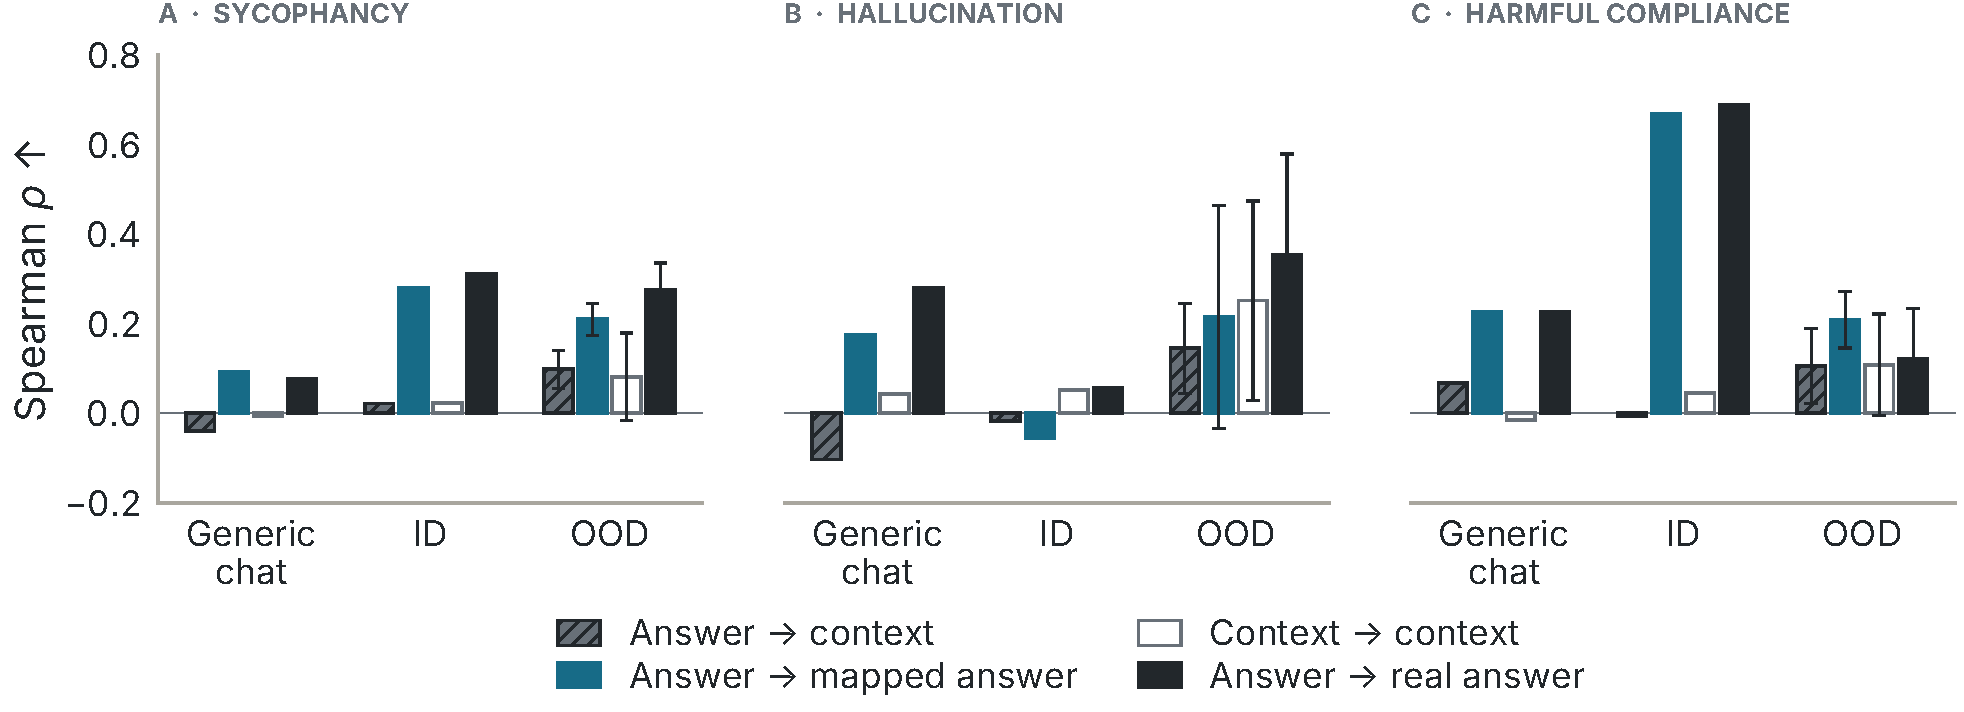
\includegraphics[width=\textwidth]{figures/paper/c5_behavior_transfer_original_combined.pdf}
    \caption{\textbf{Answer-derived readouts transfer to predicted answers and usually outperform context projections.} \panel{A} Sycophancy. \panel{B} Hallucination. \panel{C} Harmful compliance, including malicious persona and style. Each arrow names where a direction is extracted and where it is applied. Bars show Spearman correlations; OOD bars average datasets equally, with one standard error across datasets. Original behavior-augmented maps, whitening, and method-specific layers are retained. ID contexts were included in map fitting. Synthetic evaluation is excluded. Settings and limitations: \appref{app:behavior}.}
    \label{fig:behavior-prediction}
\end{figure*}
